\documentclass[12pt]{article}
\usepackage[russian]{babel}
\usepackage[utf8x]{inputenc}
\usepackage{amssymb}
\usepackage{amsmath}
\usepackage{graphicx}
\usepackage{geometry}
\usepackage[colorinlistoftodos]{todonotes}
\usepackage{listings}
\usepackage[section]{placeins}
\begin{document}

\title{2. Представление сигналов при помощи ряда Котельникова}
\author{Андрей Валиков}
\date{}
\maketitle
																																																								\section{Построение заданного сигнала}
																																																																																																													
Исходный сигнал:
\begin{gather*}
x(t) = 
\begin{cases}
  Ae^{-t/\tau} \text{ if $0\leq t\leq T_c$}\\
  0 \text{ else}    
\end{cases}
\end{gather*}

\noindent Константы имеют следующие значения:
\[A = 2\]
\[\tau = 0.5\]
\[T_c = 0.7\]

\begin{lstlisting}
N = 800
T = .3
T_max  = 1
om_max = 100

t  = np.linspace(0, T_max, N)
om = np.linspace(0, om_max, N)

n = 7

func = np.array(list(map(lambda x: _func(x, T_max), t)))
sp_1 = plt.subplot(221)
sp_1.plot(t, func, color=(0, .9, 0))
\end{lstlisting}



\section{ Расчет спектральной характеристики}
Используется тригонометрическая форма преобразования Фурье:

\[\hat{f}(\omega) = \int_{-\infty}^{\infty}x(t)\cos(\omega t)dt -
 i\int_{-\infty}^{\infty}x(t)\sin(\omega t)dt\]
 
\noindent Модуль полученной спектральной характеристики будет составлять амплитудную характеристику сигнала:
\[A(\omega) = |\hat{f}|\]


\begin{lstlisting}
amp_func = np.abs(_fourier(func, t, om))
sp_2 = plt.subplot(223)
sp_2.plot(om, amp_func, color=(0, .5, 0))
\end{lstlisting}

\begin{figure}[!htb]
\centering
\caption{}
\label{}
\end{figure}

\begin{figure}[!htb]
\centering
\caption{}
\label{}
\end{figure}

\section{ Отсчётная функция и её спектральная характеристика }

\[\phi(t) = \frac{\sin \omega_r (t-nT)}{(t-nT)} \]


\begin{lstlisting}
count_f = CDF(t, T, n)
sp_3 = plt.subplot(222)
sp_3.plot(t, count_f, color=(0, 0, .9))

fou = _fourier(count_f, t, om)
sp_4 = plt.subplot(224)
sp_4.plot(t, np.real(fou), color=(0, 0, .5))
\end{lstlisting}

\begin{figure}[htp]
\centering
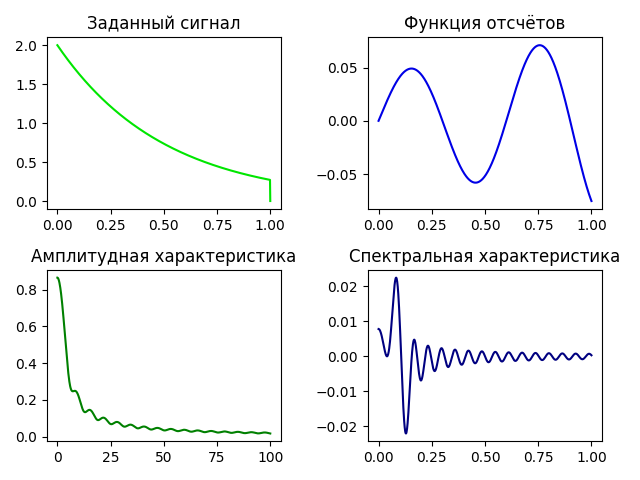
\includegraphics[scale=1.00]{first-group.png}
\caption{}
\label{}
\end{figure}

\section{ Определение граничной частоты }

\begin{lstlisting}
max_amp = .05 * max(amp_func)
for i in range(N):
  if amp_func[i] <= max_amp:
    freq = om[i]

print(freq)
\end{lstlisting}
Она оказывается равной 100.

\section{ Определение периода дискретизации и построение аппроксимирующего сигнала}



\begin{lstlisting}
T_disc = np.pi / freq
NN = int(np.fix(T_max / T_disc))

func_recovered = np.zeros(N)
for i in range(N):
  for nn in range(NN + 1):
    func_recovered[i] += _func(T * (nn - 1), T_max) * CDF(t[i], T, nn - 1)

plt.plot(t, func)
plt.plot(t, func_recovered)
plt.show()
\end{lstlisting}

\begin{figure}[htp]
\centering
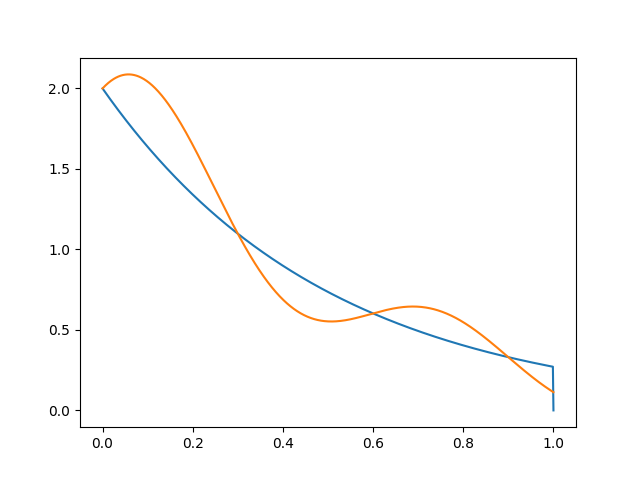
\includegraphics[scale=1.00]{compare.png}
\caption{}
\label{}
\end{figure}

\section{ Нахождение сигнала ошибки}

\begin{lstlisting}
err = abs(func - func_recovered)
\end{lstlisting}




\begin{figure}[htp]
\centering
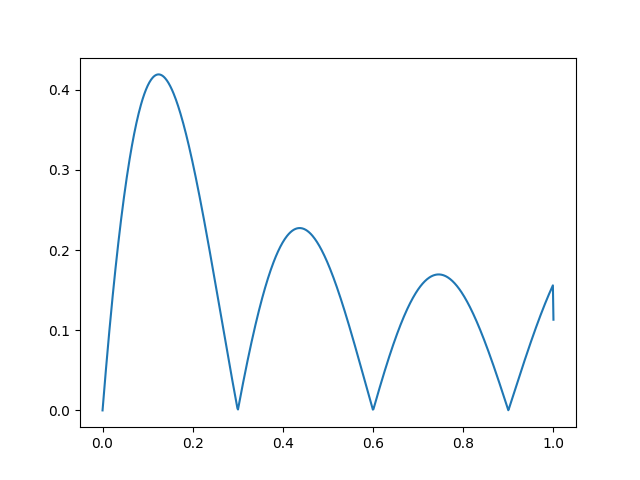
\includegraphics[scale=1.00]{error.png}
\caption{}
\label{}
\end{figure}

\section{Вывод}
Имеется исходный сигнал, экспонента на интервале [0, Tc], и нулевое значение на остальных. Используя обычное преобразование Фурье, получен комплексный Фурье образ, а на его основе, взяв абсолютное значение, амплитудную харатеристику сигнала. Далее строится отсчётная функция $sinc$. Граничная частота выбирается в два раза меньшей чем максимальная частота на спектре. Элементарной формулой определяется период дискретизации. Далее восстанавливается исходная функция.

\end{document}